\documentclass[letterpaper,11pt]{article}
\usepackage[textwidth=6.5in,textheight=8.5in]{geometry}
\usepackage{graphicx}
\usepackage{fancyhdr}
\usepackage{array}
\usepackage{amsmath}
%document font (Times)
\usepackage{tgtermes}
\usepackage[T1]{fontenc}
%\usepackage{mathptmx}
\usepackage{enumitem}
\usepackage{tabularx}
\usepackage[usenames,dvipsnames,svgnames,table]{xcolor}
\usepackage{colortbl,hhline}
\definecolor{c1}{rgb}{0.30980, 0.50588, 0.73725}
\definecolor{c2}{rgb}{0.82353, 0.87843, 0.92941}

%\hoffset=-0.74in
%\voffset= -0.8in
%\textwidth=6.5in
%\textheight=8.5in
%\marginparwidth=0pt

%\fancyhead{}
%\fancyfoot{}
%\pagenumbering{Roman}
\lhead{\includegraphics[width=0.25\textwidth]{../figures/C-3logo.png}}
\chead{Proposal Number\\A151-020-0273}
\rhead{Topic Number\\A15-020}
\cfoot{\textcopyright C-3 Comm Systems LLC. Proprietary. All Rights Reserved.}
\rfoot{\thepage}

\pagestyle{fancy}

%\title{\bf{Self-Organizing Interference Alignment (SOIA)\\for Tactical Mobile Edge Networks}}

\let\bs\boldsymbol

\begin{document}

%\thispagestyle{fancy}

%\maketitle

\begin{center}
~\\
~\\
~\\
{\Large{\huge\bf{Self-Organizing Interference Alignment (SOIA) for Tactical Mobile Ad Hoc Communications Network}}}\\
~\\
\vspace{0.1in}
Zhongren Cao\\
zcao@c3commsystems.com
\end{center}

\vspace{0.1in}

\begin{abstract}
Theoretical studies have shown the interference alignment has the potential to significantly improve the capacity of a wireless network. However, realizing interference alignment in practical networks requires costly coordination overhead, which may cancel out the gains obtained from interference alignment. In addition, it is a challenging task to group multiple transceiver pairs for interference alignment in a mobile ad hoc network where there is no centralized control.This proposal introduces self-organizing interference alignment (SOIA), a distributed approach for constructing clusters of transceiver pairs to perform interference alignment in a tactical mobile ad hoc communication network (TMACN). SOIA significantly reduces the coordination overhead by computing solutions locally at each individual receiver without requiring the channels of other receivers. SOIA leverages existing TMACN medium access control (MAC) scheme, thus it enables the seamless coexistence of  SOIA and non-SOIA radio nodes in the same network. The resulting SOIA product is expected to have low cost and supports a phased roll-out for speedy deployment without causing disruptions to existing equipment. In the proposed phase I and phase I option effort, we will develop the SOIA approach, comparatively evaluate its performance in simulation, and design a detailed Phase II prototyping and demonstration plan.
\end{abstract}

\newpage

\setcounter{page}{1}

\section{IDENTIFICATION \& SIGNIFICANCE OF THE OPPORTUNITY}

\subsection{Problem Identification}
Epitomized by recent military operations, modern warfare is conducted by small units at tactical edges. The 2012 new strategic guidance for Department of Defense articulates that one of the primary missions of the U.S. Armed forces is to project power despite anti-access/area denial (A2AD) challenges~\cite{DoD:strategy2012}, including implementing the Joint Operational Access Concept~\cite{DoD:JOAC}, which suggests ``smaller units and platforms that are rapidly deployable yet lethal." For warfighters in small units at tactical edges, efficiently sharing real-time situational awareness information is critical to their mission success. To this end, the tactical Mobile Ad hoc Communications Network (TMACN) is important because it will provide the backbone for exchange and sharing of information from sensors, manned and unmanned vehicles and systems, and dismounted soldiers. Improving the network capacity for TMACN has a direct impact on warfighter's mission success . 

%Some of the unique features that distinguish TMACNs from traditional wireless networks are their mobility; they must be self contained and have the ability to move to support forces as engagements change, their adaptability; they must be able to reconfigure themselves in real-time as new nodes are added and others are lost, and their size; they may be on the order of hundreds or even thousands of nodes. The uniqueness associated with TMACNs gives rise to several complexities that limits a satisfactory solution for performance prediction; theories required to predict their performance have yet to be developed, and adequate hardware to test them is still years away. The focus of this effort is to develop a performance prediction solution for TMACNs based on simulation.

Wireless networks are interference limited due to the fact that multiple users need to share the transmission resources. Traditionally, time and frequency resources in wireless networks are divided into orthogonal units and assigned to different users, such as TDMA, FDMA and OFDMA. Each resource unit can only be used by a single transmission in order to avoid interference among multiple simultaneous transmissions. For large networks, resource reuse is widely adopted in both commercial and military systems to increase the network capacity. The same frequency/time resource unit is shared by multiple transceiver pairs that are far apart geographically such that mutual interference is not significant due to path loss. 

In addition to the frequency and the time signaling dimensions, multiple antenna arrays and MIMO systems enable the vector space as a third signaling dimension, i.e. the spatial dimension. The spatial dimension can be shared among multiple transmissions or multiple data streams of the same transceiver pair. The same time and frequency resource unit can be shared among multiple transmissions as long as they can be separated in the spatial dimension. In the ideal case, each transmission occupies a subspace that is orthogonal to the subspaces of all other parallel transmissions. In reality, due to correlations among antennas, the channel matrix may be rank-deficient thus limits the number of simultaneous transmissions that can be supported. To some extend, spread spectrum technology can also be viewed as using vector-based signaling to support multiuser communications. 

All aforementioned approaches are built upon the basic doctrine that, in order to avoid interference, closely located transceiver pairs in a wireless network must use orthogonal transmission resource units for simultaneous transmissions. Each resource unit can only be used by a single transmission. Therefore, the number of simultaneous transmissions are upper bounded by the number of orthogonal resource units available to use. Given the limited bandwidth each radio can access and the limited number of antennas each radio is equipped per size, weight and power (SWaP) requirements, the capacity of tactical mobile networks is thus constrained during operational deployment. 

In order to further enhance the capacity of tactical networks, we need to develop fundamentally new technology that can be deployed in realistic mission operations. 

\subsection{Interference Alignment -- The Opportunity for More Wireless Network Capacity}

Interference alignment (IA) is an emerging approach, which breaks away from the above fundamental doctrine, i.e., the number of simultaneous transmissions among closely located radio transceivers is limited by the number of orthogonal transmission resource units.  

 In interference alignment, the signaling of multiple closely located transceiver pairs are jointly designed, such that at each individual receiver all interference aligned into a subspace that is orthogonal to the desired signal. The number of interferences is more than the rank of the aligned subspace. This is explained graphically in Fig.*. ... Using interference alignment, from the network point of view, the number of simultaneous transmissions within the interference range can be more than the number of available orthogonal resource units. Thus, the overall network throughput is increased.

At least in theory, shows it can significantly improve the network capacity. The theoretic concept of interference has been extensively explained in many academia publications. The theoretic framework for IA has several idealistic assumptions that need to be addressed before apply IA in practical systems. First, since IA jointly design the transmission signals for multiple transmitters, the channel state information (CSI) is central to calculating IA beamforming vectors. As a result, IA incurs significant overhead for CSI estimations and feedback. In mobile fast-fading environment, the overhead of CSI acquisition can limit or cancel out the gains of IA. 

\subsection{Practical Challenges and Requirements}

Theoretical investigation shows that a $K$-pair interference channel with IA can achieve its total DOF, which is $K/2$ [\#].  In practice, several challenges have to be addressed before materializing the capacity gain promised by IA in an operational TMACN.

{\textbf{\textit{Clustering transceiver pairs}}} --- IA requires coordination among multiple transceiver pairs to design the signals and setup the joint transmissions in the physical layer. So the first step in applying IA is to cluster transceiver pairs instead of individual nodes, as in the traditional mobile ad hoc network (MANET) clustering problem  [\#]. Even given the same group of radios, if the pairing of transceivers changes, the IA signaling of this group has to be re-designed. Most research papers discussing IA assume that the $K$ pairs are given {\it{a prior}}. This assumption is reasonable for a cellular system, where a centralized control plane manages multiple base stations and also has the full knowledge of all traffic. The knowledge of current traffic needs is necessary to determine the participating transceiver pairs within a cluster. TMACN, on the contrary, doesn't have a centralized control plane. Each radio in TMACN knows only its own traffic needs. There is no entity in a TMACN which has global knowledge of all traffic needs. In short, distributed pairing of radios with active traffic need is the first challenge to be addressed.

{\textbf{\textit{Handling heterogeneous radios}}} ---  Tactical networks are inherently heterogeneous. Dismounted soldier radios and vehicle mounted radio transceivers have different SWaP requirements. Hence, different radios are equipped with various numbers of antennas. For example, the AN/PRC-154 Rifleman Radio that is being fielded now to combat troops is a single transceiver radio. The AN/PRC-155 Manpack radio has two radio channels. More antennas may be available on vehicular-mounted radios, for example AN/PRC-117G. Given the dynamic nature of battlefield communications, the IA solution computing must take into account the fact that, within an IA cluster, some radios have reduced signal dimensionality than the others. This indicates that each radio must share its antenna configuration with neighboring nodes to facilitate transceiver pair clustering and IA solution generation. 

{\textbf{\textit{Limiting coordination overhead}}} --- To compute IA solutions, classical IA algorithms requires not only the channel state information (CSI) of all participating transceiver pairs, but also the CSI of all interfering pairs. For a $K$-pair IA scheme, $K^2$ sets of CSI information are required for computing. To control the growth of coordination overhead, smaller clusters are preferable. Since IA engine must recalculate the IA precoder beamforms when the channel changes, coordination overhead also grows in high-mobility fast-fading environment, which is typical in tactical deployment. As a result, TMACN requires IA schemes that can significantly reduce the need for CSI acquisition feedback. Protocol level coordinations, such as determining the beginning and ending of the transmission, selecting time and frequency synchronization reference point, achieving synchronization, also incur overhead. An ideal solution for practical TMACN systems would achieve protocol level coordination with minimum cost.

In addition to above challenges, inserting new technology into military systems has to be an evolutional process, such that we can not only maximize the value of existing technology and capital investment, but also speed up the deployment of new technology. Applying IA into TMACN is no exception. We need to leverage existing TMACN operations when designing the approach to cluster IA transceivers pairs, and develop the algorithm for computing IA solutions. At times when IA is unfeasible or cannot offer expected capacity gains, radios must be able to continue operate in the conventional mode.

%In particular, tactical mobile ad hoc network (TMACN) poses several challenges to apply IA. 
%Several challenges have to be addressed in order to reap the benefits of IA in operational tactical mobile ad hoc network. 
%Second, unlikely commercial systems, TMACN usually doesn't have a centralized control plane. Therefore, IA relies on distributed coordination among peer nodes. 
%Third,  technology evolution instead of revolution is better for TMACN.
%Therefore, a distributed 
%First, tactical network is inherently heterogeneous.  size weight and power (SWaP) requirements 
% Situational awareness at tactical edge requires  higher data throughput
% Interference alignment overview and its potential application to improve the throughput of tactical edge network
% General challenges of applying interference alignment 
% Challenges posed by the tactical edge networks
%  1. Hybrid nodes (vehicle node vs. dismounted nodes) from one antenna to multiple antennas
%  2. Hierarchical network architecture
% It requires several steps to incorporate IA into the TMACN operations. The first step is to identify IA opportunities. 

\section{PHASE I TECHICAL OBJECTIVES}

% A self-organizing interference alignment scheme supporting distributed clustering
% Built on the existing medium access control schemes widely adopted in TMACN.  

The overall PHASE I technical objective is to investigate, design and evaluate an interference alignment scheme, which not only can improve the capacity of TMACN, but also is practical for prototyping, demonstration and transition. Specifically, this scheme should be able to dynamically form IA transceiver clusters without a central control plane,  operate flexibly with heterogeneous radio nodes, and significantly reduce coordination feedbacks. There are four technical objectives for the Phase I effort including the Phase I option. These objectives are
\begin{itemize}[noitemsep,nolistsep]
\item{Design Self-organizing Interference Alignment (SOIA) for Tactical Networks}
\item{Evaluate System Performance}
\item{Develop Protocol Frame Structure}
\item{Plan Phase II Prototyping and Demonstration}
\end{itemize}
In the following sections, the above four technical objectives are described in detail. 

%The objectives of this proposal to develop a practical interference alignment scheme that is applicable to transmission scheme 

%In we propose to design a software suite, which enables distributed interference alignment cooperations among tactical edge mobile nodes.  Since most existing military waveforms operate in slotted or TDMA mode, THE SYSTEM assumes a operational slotted network without IA as the baseline. In order to be backward compatible with existing tactical protocols,  where initial slot assignment is assumed to be performed by methods used in existing TMACN, such as SRW. Thus, each node possesses a series of time slots. The system level gain from IA comes from enabling other transceiver pairs to share time slots assigned to node ??. 

\subsection{Design Self-organizing Interference Alignment (SOIA) for Tactical Networks}

Interference alignment leverages the fact that interference signals, unlike noise, have inherent structures as they are generated by other radio transmitters to carry information. If multiple interfering signals at a receiver are all structured to match a subspace that is orthogonal to the subspace of the desired signal(s) of the receiver, these interfering signals are aligned without deteriorating the reception of the desired signal. 

\subsubsection{TMACN Requirements for Interference Alignment}

IA usually finds its uses in $K$-user interference channel and X-channels. The typical application scenario for IA in TMACN is the $K$-user interference channels. Most algorithms for computing IA precoders and equalizers assume the clustering of transceiver pairs are given. An IA cluster is determined by the set of participating nodes,  the pairing among these nodes, and the traffic directions for each pair of nodes. TMACN doesn't have a central control plane. Therefore, an IA cluster in TMACN has be formed in a distributed way. Furthermore, the topology of a TMACN is dynamic since nodes are mobile. The constituent members of each cluster are dynamic with existing nodes leaving an cluster and new nodes joining. To this end, IA clusters in SOIA are transient, i.e., clusters are formed and dissolved quickly. Transient clusters are particularly suitable for IA. An IA solution not only depends on the members of an cluster, but also the channels among the cluster members. If some change changes, a new IA solution has to be computed. The optimum solution may require dropping some pairs of transceivers and adding new pairs. In other words, after channel changes, essentially a new cluster is required with a new IA solution over a different set of transceiver pairs. 

\subsubsection{Cluster Head Pair Identification}

To form a transient IA cluster in a distributed way, it is necessary to identify the cluster head efficiently in a simple manner. In SOIA, the simplicity is achieved by seamlessly integrating the cluster head identification with existing TMACN medium access control scheme. TDMA is the popular choice among TMACN tactical waveforms for multiuser medium access management. For example, SRW has a centralized TDMA resource management within each island (a group of radio nodes); WNW uses distributed TDMA with dynamic slot allocations. The proposed SOIA scheme will use the time slots assignment schemes of existing TMACN tactical waveforms. Specifically, when a node $A$ is assigned with a set of time slots in a TDMA frame, and node $A$ decides to use these slots to transmit information to node $B$, in SOIA node $A$ automatically assumes the head position of a potential IA cluster spanning these time slots with the pair of nodes $A$ and $B$ as the head pair.  There are two folds of benefits SOIA provides by leveraging existing TMACN time slots assignment schemes.
\begin{itemize}[noitemsep,nolistsep]
\item SOIA simplifies IA technology insertion and assures the system is backward compatible. There is no need to reinvent a complete communication protocol stack. Instead, SOIA can be realized as add-on software and firmware modules, which can be easily inserted into existing programmable radio systems. When the channel condition doesn't warrant the gain of using IA, the radios can smoothly revert back to non-IA operations since the same MAC frame slots assignment is used. Furthermore, SOIA supports radio deployment in phases by enabling the mix of radios with and without IA capabilities inside the same TMACN. Again, this is because that all radios follow the same slot assignment schemes.
\item SOIA designates the IA cluster head unambiguously without coordination overhead. As shown in Fig.~\ref{fig:IA_SingleRx}, the MAC control assigns the time slot $t_n$ to the transmission of radio node 2. Node 2 decides to transmit to radio node 1, based on its own application needs. In SOIA, this transceiver pair, i.e., node 1 \& 2, is called is called the ``head pair" of the IA cluster for time slot $t_n$. Identifying the ``head pair" of an IA cluster is the critical first step in the SOIA scheme. Note at this moment, it is unclear which of the other possible transceiver pairs would join the cluster to transmit in slot $t_n$. SOIA simplifies the clustering strategy by identifying the cluster ``head pair" without adding {\textbf\textit{any}} coordination overhead to the existing slot assignment scheme.
\end{itemize}

\begin{figure}[h]
\begin{center}
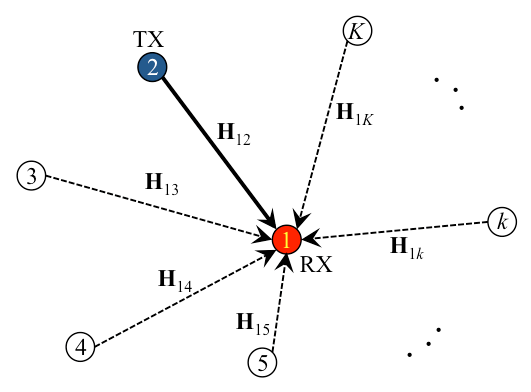
\includegraphics[width=0.5\textwidth]{../figures/InterferenceAlignment_1.png}
\caption{\small Self-organizing interference alignment (SOIA) illustrations. Blue node $t$, which is assigned with transmission slots by TMACN TDMA, selects red node $r$ as the receiver. The pair of nodes $t$ and $r$ automatically assumes the role of head pair for a transient IA cluster. All nodes in the network not only tracks the spatial channel from its neighbors, but also the interference subspace signature from all recent transmission pairs among neighbors. Three potential pairs are illustrated.}
\label{fig:IA_SingleRx}
\end{center}
\end{figure}

\subsubsection{Local Interference Alignment}\label{LocalIA}

With the cluster head pair given, the next step in SOIA is to select other transceiver pairs from the neighborhood. These other pairs should be able to transmit at the same time with the head pair. Jointly, these simultaneous transmission pairs form an IA cluster.  An idealistic IA solution requires the channel knowledge from each transmitter of a cluster to all receivers in the same cluster. The precoders for each transmitter are jointly designed. Obviously, the overhead associated with idealistic IA solutions is too expensive for practical TMACN operations. In addition, idealistic IA solutions assume working in high SNR. For practical TMACN with moderate to low SNRs, maximize receiver SNR should be considered.

In SOIA, the interference among all pairs are locally aligned at the head pair receiver first with the goal to maximize the receiver SNR. Compared to idealistic IA solutions, this approach can significantly reduce overhead resources. The head pair receiver can compute a local IA solution based on its estimated channels without considering the channels seen by other receivers. As an example, in Fig.~\ref{fig:IA_SingleRx}, the pair of node $t$ and node $r$ is the current head pair, in which node $t$ is the transmitter and node $r$ is the receiver. It is reasonable to assume that each radio node in TMACN keeps track of its neighbors and the channels from these neighbors to itself. The estimates of these channels can be acquired and kept up-to-date locally. In Fig.~\ref{fig:IA_SingleRx},  node $r$ has $N$ neighboring nodes besides node $t$. Let ${\bf{H}}_{rk}$ denote the channel between node $k$ and node $r$. Node $r$ can keep track of ${\bf{H}}_{rk}$ by performing channel estimations based not only on periodic beacon signals sent by node $k$, but also on any signal sent by node $k$ regardless of whether node $r$ is the intended recipient. 

The algorithm for local IA is given in the following using node $r$ in Fig.~\ref{fig:IA_SingleRx}. Considering the heterogeneous radio configuration in TMACN, we assume that node $t$ has $n_t$ antennas and node $r$ has $n_r$ antennas. Based on channel $\mathbf{H}_{rt}$, node $r$ first selects the number of data streams $S_r$ that node $t$ can send to it. Then, node $r$ computes the precoder matrix $\mathbf{B}_{r,t}=[\bs{b}_{r,t,1}~\bs{b}_{r,t,2}\cdots~\bs{b}_{r,t,S_r}]$ for node $t$ such that the received SNR is maximized. If node $t$ sends only a single data stream to node $r$, $S_r=1$ and $\mathbf{B}_{r,t}=\bs{b}_{r,t,1}$.

Maximize the SNR for the received signal is equivalent to
\begin{equation}\label{bfCapacity}
C=\displaystyle\max_{{\mathbf{B}}_{r,t}}\log\left|\mathbf{I}_{S_r}+\frac{\mathbf{B}_{r,t}^{*}\mathbf{H}_{rt}^{*}\mathbf{H}_{rt}\mathbf{B}_{r,t}}{\sigma^2}\right|
\end{equation}
where $\sigma^2$ is the noise power at receiver $r$. In Eq. (\ref{bfCapacity}), node $r$ calculates the transmitter precoder matrix for node $t$, which maximizes the capacity between node $r$ and node $t$. The columns of the resulting $\mathbf{B}_{r,t}$ are the eigenvectors corresponding to the largest $S_r$ eigenvalues of matrix $\boldsymbol{\Phi}=\mathbf{H}_{rt}^{*}\mathbf{H}_{rt}$.

Node $r$ feeds back the matrix $\mathbf{B}_{r,t}$ to node $t$. The feedback overhead can be further reduced if using vector quantization methods. In addition, if the assumption of channel reciprocity holds true for the tactical radios in tactical operations, the need for feedback $\mathbf{B}_{r,t}$ can be eliminated as $\mathbf{H}_{rt}=\mathbf{H}^{*}_{tr}$. Therefore, node $t$ can compute the precoder matrix $\mathbf{B}_{r,t}$. However, in SOIA, it is necessary for node $r$ to have knowledge of $\mathbf{B}_{r,t}$. The reasons are explained in Section~\ref{member_selection}.

%that maximizes $C$ is the one that maximizes the quadratic form $|\boldsymbol{v}_2^*\boldsymbol{\Phi}\boldsymbol{v}_2|$, where  So $\boldsymbol{v}_2$ is the eigenvector corresponding to the largest eigenvalue of $\boldsymbol{\Phi}$. Node 1 sends $\boldsymbol{v}_2$ to node 2 so the latter will use it as the transmitter beamforming vector. The desired signal space of node 2 is thus given by $\mathbf{H}_{12}\boldsymbol{v}_2$. 

%in the following that each radio has only 2 antennas. So, out of the 2 dimensional vector space each radio, one dimension is the signal space of the radio while the other is the interference space. To align the transmissions of all neighbors, node 1 computes the transmission precoder beam forming vectors ${\boldsymbol{v}}_k$ for node $k=2, 3, \cdots, K$ such that

%and
%\begin{equation}\label{nullbfvec}
%\boldsymbol{v}_k^{*}\mathbf{H}_{1k}^{*}\mathbf{H}_{12}\boldsymbol{v}_2=\mathbf{0}, {\rm{for}}~k=3,4,\cdots~K.
%\end{equation}


%In the next step, node 1 computes the beamforming vectors for all other potential interference sources in its neighborhood, i.e., node 3, 4, $\cdots~K$. More specifically, node 1 aligns all potential interference in the subspace that is orthogonal to its desired signal space. Let $\boldsymbol{v}_k$ be the transmitter beamforming vector for node k. Node 1 computes $\boldsymbol{v}_k$ such that Eq.~(\ref{nullbfvec}) holds true for nodes 3, 4, $\cdots~K$. Node 1 will broadcast vectors $\boldsymbol{v}_3$, $\boldsymbol{v}_4$, $\cdots$ $\boldsymbol{v}_K$ along with $\boldsymbol{v}_2$. Therefore, every node in the neighborhood of node 1 not only knows its own beamforming vector, but also the beamforming vector of all other nodes.

%Without IA coordination, nodes 3, 4, $\cdots~K$ cannot transmit during the time slots assigned to node 2, which will use these slots to send information to node 1. By computing and broadcasting beamforming vectors $\boldsymbol{v}_3$, $\boldsymbol{v}_4$, $\cdots$ $\boldsymbol{v}_K$, node 1 provides an opportunity for some of these nodes to join the transient IA cluster headed by node 1 and 2 without impacting the transmission from node 2 to node 1. 

\subsubsection{Cluster Member Selection}\label{member_selection}
 
After having designated the head pair of a transient cluster and designed the precoder matrix for the head pair transmitter to maximize the SNR at the receiver, SOIA proceeds to select other transceiver pairs in the neighborhood that can operate at the same time as the head pair. The receiver node $r$ of the head pair for current time slots leads the selection process. Let $\mathcal{U}=\{1, 2, \cdots, U\}$ be the set of all active neighboring transceiver pairs seen by node $r$. For example, three potential pairs are illustrated in Fig.~\ref{fig:IA_SingleRx}. A neighbor node may be associated with more than one potential pair to be considered. In Fig.~\ref{fig:IA_SingleRx}, node $l$ and node $j$ are a potential pair of nodes; node $l$ and node $m$ are another pair of nodes. Both pairs are being evaluated by node $r$ as possible cluster members.
%Since node 1 broadcasts the precoder beamforming vectors  $\boldsymbol{v}_2$, $\boldsymbol{v}_3$, $\cdots$ $\boldsymbol{v}_K$, each neighbor node not only knows its own transmission vector, but also the transmission vectors of all other nodes. Node 3, 4, $\cdots$, $K$ use this knowledge to determine whether it can, as a receiver, join the transient IA cluster headed by node 1 and 2, and also determines the transmitter node at the same time. %Node $l$, similar to node 1, keeps track of $\boldsymbol{H}_{lk}$ by performing channel estimations based not only on periodic beacon signals sent by node $k$, but also on any signals sent by node $k$ regardless whether node $l$ is the intended recipient. Therefore, node $l$ can calculate the local subspace occupied by the interference from node 1, which is $\boldsymbol{H}_{l1}\boldsymbol{v}_{1}$.  Similarly, the local subspace occupied by potential signals from node $k$ is given by $\boldsymbol{H}_{lk}\boldsymbol{v}_{k}$.

SOIA reuses existing MAC slots assignment schemes. The node with assigned slots automatically assumes the cluster head position of a transient IA cluster. Hence, every pair of nodes with on-going traffic have the opportunity to lead its own transient IA cluster within a TMACN TDMA frame. Let's assume that each pair of nodes in $\mathcal{U}$ has on-going traffic and is active within recent TDMA frames. Let $\mathbf{B}_{j,l}$ denote the precoder matrix the transmitter node $l$ uses for the receiver node $j$, when node $l$ is assigned with time slots to transmit and the pair of nodes $l$ and $j$ is the cluster head. According to Section~\ref{LocalIA}, $\mathbf{B}_{j,l}$ maximizes the received SNR at node $j$ for signals from node $l$. $\mathbf{B}_{j,l}=[\bs{b}_{j,l,1}~\bs{b}_{j,l,2}\cdots~\bs{b}_{j,l,S_{j}}]$, where $S_{j}$ is the number of data streams node $l$ sends to node $j$.  

For a neighbor node $k$, let $\mathbf{H}_{k,l}$ be the channel between the node $l$ and node $k$. The transmission from node $l$ to node $j$ causes interference at node $k$ with its subspace signature given by
\begin{equation}
\mathbf{P}^{[k]}_{j,l}=\mathbf{H}_{k,l}\mathbf{B}_{j,l}.
\end{equation}
For any node $k$, $k\neq j$ and $k\neq l$, $\mathbf{P}^{[k]}_{j,l}$ can be estimated by
\begin{equation}\label{equ:estimate_interference_signature}
\hat{\mathbf{P}}^{[k]}_{j,l} = \mathbf{Y}_{k,l}\mathbf{X}_l^{-1}=\left(\mathbf{H}_{k,l}\mathbf{B}_{j,l}\mathbf{X}_l+\mathbf{N}_k\right)\mathbf{X}_l^{-1}=\mathbf{H}_{k,l}\mathbf{B}_{j,l}+\mathbf{N}_k\mathbf{X}^{-1}_l.
\end{equation}
In Eq.~(\ref{equ:estimate_interference_signature}),  $\mathbf{X}_l$ is a training structure used known to all nodes. $\mathbf{Y}_{k,l}$ is the training signal received by node $k$ from node $l$. In Section~\ref{sec:frame_and_protocol}, the IA subframe structure is introduced, where a dedicated interference training period is inserted. During this interference training period, only node $l$ transmits. Therefore, each node in $l$'s neighbor can estimate the interference subspace signature it sees from the transmission from $l$ to $j$. It is worthwhile to point out several useful features of the definition for interference subspace signature in Equ.~(\ref{equ:estimate_interference_signature}).
\begin{itemize}[noitemsep,nolistsep]
\item Interference power has been implicitly incorporated in the definition of $\hat{\mathbf{P}}^{[k]}_{j,l}$, if we assume the symbol column energy in $\mathbf{X}$ is fixed to unit. 
\item The training symbol matrix $\mathbf{X}_l$ is an $S_j$ by $S_j$ square matrix. For IA operations, $S_j<n_j$, where $n_j$ is the number of antennas on node $j$. In practical TMACN operations, the number antennas on each radio is limited. Thus, a limited set of training symbol matrices can be pre-installed onto each radio. Node $l$ broadcasts $S_j$ to all its neighbors such that node $k$ is able to select the correct training symbol matrix to estimate $\hat{\mathbf{P}}^{[k]}_{j,l}$. Section~\ref{sec:frame_and_protocol} provides details on the protocol frame structure in which $S_j$ is included in the header information.
\item More importantly, Equ.~(\ref{equ:estimate_interference_signature}) supports heterogenous antenna configurations among different nodes. This is particularly useful for TMACN operations with heterogeneous radio nodes. The matrix  $\hat{\mathbf{P}}^{[k]}_{j,l}$ has $n_k$ rows and $S_j$ columns. $n_k$ is the number of antennas on node $k$. The number of antennas on node $l$ is irrelevant since $n_l$ is absorbed by the inner product of $\mathbf{H}_{k,l}$ and $\mathbf{B}_{j,l}$. Therefore, regardless of the number of antennas on nodes of the interference source, all interference subspace signature at a node has the same number of rows. 
\end{itemize}

Using the sub frame structure introduced in Section~\ref{sec:frame_and_protocol}, the receiving node of the cluster head pair, node $r$, is able to keep track of $\hat{\mathbf{P}}^{[r]}_{j,l}$ for all potential transceiver pairs $\mathcal{U}$ among its neighbors. As we indicated in Section~\ref{LocalIA}, $r$ has to be aware of the precoder matrix $\mathbf{B}_{rt}$ for its own transmitter node $t$ and the channel $\mathbf{H}_{rt}$ between node $t$ and node $r$. Both can be obtained locally by node $r$. Thus, node $r$ is able to locally compute the signal subspace from node $t$ as $\mathbf{S}_{rt}=\mathbf{H}_{rt}\mathbf{B}_{rt}$. In addition, node $r$ is able to calculate the projection of the interference subspace of all potential transceiver pairs in $\mathcal{U}$ onto the signal subspace $\mathbf{S}_{rt}$. For the pair $u\colon=\{l\rightarrow j\}$, its projected interference energy over $\mathbf{S}_{rt}$ is given by the norm of the projection in the following equation.
\begin{equation}\label{projection}
A^{u}_{rt}=\left\Arrowvert\left(\mathbf{P}^{[r]}_{l,j}\right)^{*}\mathbf{S}_{rt}\right\Arrowvert_{2}~\textrm{for~any~}u\in\mathcal{U}.
\end{equation}
The member pairs node $r$ selects for the transient cluster headed by node pair $r$ and $t$ are those pairs in $\mathcal{U}$ whose interference subspace signatures project lower energy onto the signal subspace $\mathbf{S}_{rt}$.  During phase I, we plan to evaluate the following two approaches for cluster member selection.

\noindent{\textbf{Centralized selection at node $r$ based on a threshold}} 

In centralized selection, node $r$ selects pair $u\in\mathcal{U}$ as the the cluster member if  $A^{u}_{rt}\le\theta$, where $\theta$ is a threshold. We will evaluate and determine the threshold $\theta$ given different operational scenarios during the Phase I effort. The members of the IA cluster headed by transceiver pair $t$ and $r$ are 
$$
\mathcal{W}=\{w\colon={t\rightarrow r}\}\cup \tilde{\mathcal{U}},
$$
where
\begin{equation}\label{tilde_U}
\tilde{\mathcal{U}} = \left\{ A^{u}_{rt}\le\theta, u\in\mathcal{U} \right\}.
\end{equation}
Each node can only be associated with a single pair. It is possible that multiple transceiver pairs with overlapping nodes all meet the above threshold based selection criterion. As an example, in Fig.~\ref{fig:IA_SingleRx}, both the pair of nodes $l$, $j$ and the pair of node $m$, $l$ are selected by node $r$. So node $l$ appears in both selected pairs. Node $r$ select the node $j$ to pair with $l$ if $A^{u}_{rt} < A^{v}_{rt}$, where $v\colon=\{l\rightarrow m\}$.

Node $r$ informs its neighbors the selection of its cluster member pairs $\tilde{\mathcal{U}}$. Each pair being selected has to determine its transmission strategy. While the SOIA strategy for the head pair $\{w\colon={t\rightarrow r}\}$ is to maximize the SNR for the received signal at node $r$, the SOIA strategy for all pairs in $\tilde{\mathcal{U}}$ is to minimize the interference power. 

Let's assume the pair $u\colon=\{l\rightarrow j\}$ is one of the selected pairs, in which $l$ is the transmitter and $j$ is the receiver. Similar to node $r$, node $j$ keeps track of the interference subspace signature it sees from all active transceiver pairs in its neighborhood $\mathcal{V}={1, 2,\cdots,V}$. Let $\mathcal{Z}={\mathcal{W}}\cap\mathcal{V}$. Transceiver pairs in ${\mathcal{W}}$ but not in ${\mathcal{Z}}$ are not neighbors for node $j$, hence the interference from those transceiver pairs is negligible for node $j$. Therefore, the received signal of $j$ is
\begin{equation}\label{rx_sig}
\displaystyle\boldsymbol{y}^{[j]}=\mathbf{H}_{jl}\mathbf{B}_{jl}\bs{s}_{jl}+\sum_{\substack{z\in\mathcal{Z}\\z\neq u}}\mathbf{P}^{[j]}_{z}\bs{s}_z+\bs{n}_r.
\end{equation}
To minimize the interference power, the equalizer node $j$ uses for the IA cluster headed by nodes $t$ and $r$, $\mathbf{\Pi}^{[rt]}_j$, is composed of eigenvectors corresponds to the lowest $S_j$ eigenvalues of matrix
\begin{equation}\label{}
\mathbf{\Phi}=\sum_{\substack{z\in\mathcal{Z}\\z\neq u}}\mathbf{P}^{[j]}_{z}\left(\mathbf{P}^{[j]}_{z}\right)^{*}.
\end{equation}

\noindent{\textbf{Cascaded selection}}

Cascaded selection is the second approach that we plan to investigate during the phase I effort for cluster member selection. Similar to the centralized selection, in cascaded selection the receiver node of the cluster head pair $r$ first determines the set $\tilde{\mathbf{U}}$ according to Eq.~(\ref{tilde_U}). Different from the centralized approach, rather than selecting all pairs in $\tilde{\mathcal{U}}$ as members of the cluster, node $r$ chooses only one pair of nodes from $\tilde{\mathcal{U}}$ with the least interference energy projection. In other words, node $r$ selects pairs $u$ as the second member of the IA cluster according to
$$
\min_{u\in{\tilde{\mathcal{U}}}}A^{u}_{rt}.
$$
Node $r$ broadcasts the selection of pair $u$ as well as $\tilde{\mathcal{U}}$ to all its neighbors. In the next step,  the receiver node of $u$, node $j$, select the third pair according to 
$$
\min_{\substack{z\in{\tilde{\mathcal{Z}}}}\\z\neq w}A^{z}_{jl}~~~~\textrm{and}~~~~~A^{z}_{jl}<\theta
$$
In other words, node $j$ selects the third pair for the IA cluster from the joint set $\mathcal{Z}$. The chosen pair $z$ has the least interference energy projection onto node $j$'s signal subspace. Node $j$ broadcast it selection. This process continues until no more pairs can be selected. For all chosen pairs except the head pair, the receiver nodes computes the equalizer matrices using the same method introduced in the centralized selection scheme.

The SOIA approach is designed to materialize the capacity gain of interference alignment in practical tactical network operations with realistic moderate SNR for communication links. The SOIA approach emphasizes maximizing SNR for the cluster head pair while minimizing interference power for non-head pairs in an IA cluster. In particular, SOIA solutions are computed distributedly with only local channel knowledge. Therefore, SOIA significantly reduces the coordination overhead and is practical for real world tactical network operations.

\subsection{Evaluate System Performance}

During the Phase I effort, we plan to model the SOIA approach in MATLAB and develop MATLAB-based simulator to evaluate the SOIA system performance. The SOIA team recognizes that it is extremely important to have a high fidelity physical layer propagation model in order to evaluate the SOIA system performance. Many networking simulation tools, such as Qualnet and OpNet, have na�ve physical layer models. The SOIA team has extensive experience in realistic MIMO channel modeling and in using Ericsson's RUNE (Rudimentary Network Emulator)~\cite{ZandRRM:book:2001}, a MATLAB-based TDMA wireless networking simulation tool available to public. We will incorporate many features of RUNE into the SOIA performance simulation.

\subsubsection{Spatial Channel Models for MANET}

Accurate physical layer MIMO channel modeling is critical for simulation based TMACN evaluation. During Phase I effort, we will adopt and adapt the industry standard MIMO spatial channel model, the 3GPP spatial channel model (SCM) for MIMO simulations~\cite{3GPP:SCM}.  The SOIA team has prior experience implementing 3GPP SCM in MATLAB under the Ericsson RUNE framework. 

The 3GPP SCM was developed for cellular network simulation. However, by lowering the antenna height, we could easily convert it into system level simulation for mobile ad hoc networks. For a given laydown of $N$ radio nodes, the planned simulator will generate a $N-1$ by $N-1$ path gain matrix between all possible transceiver pairs. The fast fading MIMO coefficients will be generated according to the 3GPP SCM. The path gain between any pair of radios is the sum of the distance-based path loss and the lognormal shadowing. For the distance based path loss, similar to the 3GPP Spatial Channel Model~\cite{3GPP:SCM}, we will use the COST 231 Walfish-Ikegami NLOS and LOS models. The lognormal shadowing for the NLOS has a standard deviation of 10dB, and that for LOS is 4dB, as given in~\cite{3GPP:SCM}. Furthermore, for the same transmitter, two closely located receivers have correlated lognormal shadowing. We use a pre-generated correlated lognormal map, from which each tactical receiver?s lognormal shadowing can be derived based on its location. Fig.~\ref{fig:lognormalmap} shows an example of correlated lognormal shadowing map over an area of 300 meters by 300 meters.

\begin{figure}[h]
\begin{center}
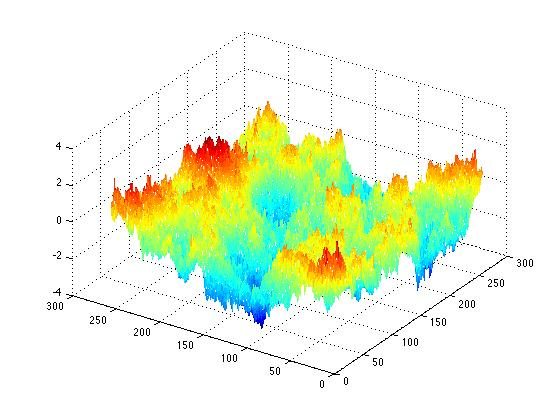
\includegraphics[width=0.66\textwidth]{../figures/lognormalmap.jpg}
\caption{\small An example of correlated lognormal shadowing map over an area of 300 meters by 300 meters. The unit for the vertical axis is dB.}
\label{fig:lognormalmap}
\end{center}
\end{figure}

\subsubsection{Mobility Trace}

Due to tactical radio mobility, the channel and the path loss between any pair of transmitters changes slot by slot.  In Phase I simulation, we assume that the platoon is patrolling in an urban area. We use a complex value (in other words, a 2-dimensional vector) to represent node speed, in which the L2 norm of the complex value represents the absolute value of the speed (m/s); and the direction of the complex value represents the mobility direction. For each slot, changes in the speed and its direction of each radio are randomly generated based on the average speed and acceleration of each radio. As a result, each radio will have a new position in the 2-D plan for every TDMA slot. The new positions are then used in the physical channel model to calculate the received signal strength at each tactical radio from all potential transmitters. 

The mobility traces not only can be randomly generated from the Matlab simulator, but also can be incorporated from real operation collections as well as Google Earth KML files. This feature enable us to evaluate the SOIA system performance in a realistic tactical maneuver.

%\subsubsection{System Performance Metric}

\subsection{Develop Protocol Frame Structure}\label{sec:frame_and_protocol}

To the end, at the protocol level, a training signal has to included during the transmission from $l$ to $j$, during which no other IA participa  

\subsection{Plan Phase II Prototyping and Demonstration}

\section{PHASE I WORK PLAN}

\section{RELATED WORK}

Since the introduction, interference alignment has attracted the attention of many researchers from around the world. Numerous research papers have been published, from which we can draw insights into this technology. However, many of these papers focus on the theoretic study of interference alignment scheme and capacity gain in high SNR range, and assume that the clustering of transceiver pairs are given a prior. Applying IA into practical communication system is still an challenging issue.

Several recent papers investigated the issue of applying IA in cellular network [][]. Note that reference [] is published by Professor Bhaskar Rao, who is consultant of C-3 Comm Systems on this proposal. Applying IA in cellular networks is relatively convenient since cellular systems have centralized control plane and high-speed wired network connecting base stations. Therefore, cellular systems are able to aggregate the channel knowledge of all users for optimum user clustering and computing IA solution. The same cannot be said for tactical mobile ad hoc networks. In general, TMACN doesn't have a centralized control plane. Furthermore, TMACN usually operates in low to moderate SNR range. Interference alignment has to be considered jointly with SNR enhancement. Therefore, applying IA to TMACN network is very challenging. In addition, prototyping IA schemes in tactical software defined radio platforms with MIMO capability further increase the difficulty of this SBIR topic.

The PI at C-3 Comm Systems brings a combined expertise on the operation of tactical networks and software defined radio system prototyping. These combined experience position C-3 Comm Systems as a strong contender to fulfill the requirements of this SBIR topic and deliver to Army a working demonstration of TMACN operating with interference alignment.

\begin{table}
\caption{default}
\begin{center}
\begin{tabular}{|>{\arraybackslash}p{\textwidth}|}
\hline
\rowcolor{c1}{
\begin{tabular}{@{}l@{}}
\color{white}{\textbf{Project: Content-Based Mobile Edge Networking (CBMEN)}}\\ 
\color{white}{\textbf{Sponsor: DARPA}}\\ 
\end{tabular}}\\
\hline
\rowcolor{c2} {\textbf{Project Summary:}} Dr. Cao (C-3 Comm Systems) was a senior personnel on the USC/ISI mobile system integrators (MSI) team for the CBMEN program, which developed algorithms for content storage, distribution, and access at the tactical edge by small unit warfighters.  Dr. Cao led USC/ISI's effort to establish an EMANE-based networking emulation lab with multiple high-end Linux servers and more than 150 Android phones. Furthermore, Dr. Cao planned and executed a month long large-scale field test and demonstration event for the Phase I CBMEN program at Ft. A. P. Hill. In this event, USC/ISI designed and deployed a platoon size heterogeneous MANET network over a 2 kilometers long hilly range, using both Rifleman radios and commercial-off-the-shelf (COTS) Android phones. \\
\hline
{\textbf{Relevance to SOIA:}} \\
\hline\hline
\end{tabular}
\end{center}
\label{default}
\end{table}%
 

\section{RELATIONSHIP WITH FUTURE RESEARCH OR RESEARCH AND DEVELOPMENT}

\section{COMMERCIALIZATION STRATEGY}

\section{KEY PERSONNEL}

\subsection{Principal Investigator --- Zhongren Cao, Ph.D.}
Dr. Cao is the founder and owner of C-3 Comm Systems, LLC. He is a United States permanent resident. He will lead the investigation effort during Phase I and Phase I Option. 

Dr. Cao earned his Ph.D. degree in electrical engineering from Stevens Institute of Technology in 2004. He obtained his M.E. degree from Shanghai Jiaotong University in 2000 and his B.S. degree from Xi'an Jiaotong University in 1997, both in electrical engineering. Since March 2012, Dr. Cao has been a research scientist in the wireless networking group at the Information Sciences Institute (ISI), University of Southern California (USC). From 2004 to 2012, Dr. Cao was a senior research staff and project leader at the University of California, San Diego Division of the California Institute for Telecommunications and Information Technology (Calit2). 

Dr. Cao's technical expertise spans across wireless communications and networking systems, signal processing algorithms and software defined radio (SDR) system prototyping using heterogeneous computing platforms. His research targets at creating and implementing innovative wireless networking system concepts to enable new applications and improve the system performance and efficiency. In USC/ISI, he  led the technical development, large scale emulation, field-testing and demonstration for the DARPA CBMEN program. He successfully organized a month-long DARPA CBMEN field tests and demonstration. This is a large scale tactical mobile ad hoc network demonstration using Program of Record tactical radios and smart phones in a multi-kilometer tactical range. Dr. Cao demonstrated that using content-oriented networking technology can significantly improve the system level performance of tactical mobile ad hoc networks. In Calit2, he established the Wireless Communication System Prototyping Lab. He was the project leader or the senior personnel in several projects on wireless networking and communication system prototyping. His sponsors include DoD, Ericsson, etc. He led his team to successfully develop an FPGA based OFDM modem system-on-chip (SoC).  Using the SoC, he demonstrated innovative wireless networking system concepts, such as Coordinated Multi-Point (CoMP) and Device-to-Device, in both Calit2 and Ericsson Research in Stockholm, Sweden. Dr. Cao publishes in wireless communications and software defined radio prototyping and demonstration. His journal and conference papers are well cited by other researchers.  

\subsubsection{Relevant Publications}
Dr. Cao's publications that are relevant to subspace-based signal processing for MIMO and OFDMA systems are listed in the following.
\begin{enumerate}[topsep=0pt,itemsep=-1ex,partopsep=1ex,parsep=1ex]
\item Z. Cao, U. Tureli and Y.D. Yao, ``Low-complexity orthogonal spectral signal construction for generalized OFDMA uplink with frequency synchronization errors," in IEEE Transactions on Vehicular Technology, vol.56, no. 3, pp.1143-1154, May 2007.
\item D. Radovic, Z. Cao and M. Eric, ``Performance Analysis of the Multi-User Interleaved OFDMA Uplink Receiver in the presence of Carrier Frequency Offsets", in Proceedings of the 9th International Symposium on Wireless Personal Multimedia Communications, September 2006.
\item P. Honan, Z. Cao and T. Tureli, ``Adaptive Reduced-Rank MIMO Decoder for Military Communications", in Proceedings of the 2006 IEEE Military Communications Conference (MILCOM 2006), October 2006.
\item	D. Radovic, Z. Cao and M. Eric, ``Effects of Uplink Channel on Multi-User Interleaved OFDMA Synchronization Receiver Performance", in Proceedings of the 11th International OFDM Workshop, August 2006.
\item	P. Honan, Z. Cao and T. Tureli, ``Adaptive Reduced-Rank Interference Suppression for MIMO Decoding," in Proceedings of International Conference on Digital Telecommunications (ICDT'06), August 2006.
\item Z. Cao, U. Tureli and Y. D. Yao, ``Frequency synchronization for generalized OFDMA uplink," in Proceedings of IEEE Global Telecommunication Conference (Globecom?04), vol.2, pp.1071-1075, December 2004. 
\item	Z. Cao, U. Tureli and Y. D. Yao, ``Deterministic multiuser carrier frequency offset estimation for interleaved OFDMA uplink," in IEEE Transactions on Communications, vol. 52, no. 9, pp.1585-1594, September 2004.
\item Z. Cao, U. Tureli, Y. D. Yao and P. Liu, ``Optimum Subcarrier Assignment for OFDAM Uplink," in Proceedings of the 37th IEEE Asilomar Conference on Signals, Systems and Computers, vol.1, pp.708-712, November 2003.
\item	Z. Cao, U. Tureli and Y. D. Yao, ``Efficient Structure-based Carrier Frequency Offset Estimation for Interleaved OFDMA Uplink," in Proceedings of IEEE International Conference on Communications (ICC'03), vol.5, pp.3361 - 3365, May 2003.
\end{enumerate}

\noindent{Dr. Cao's publications that are relevant to {\bf{wireless system prototyping}}, {\bf{software defined radio methodology}} and {\bf{demonstrations of innovative wireless system concepts}} are listed in the following.}
\begin{enumerate}[topsep=0pt,itemsep=-1ex,partopsep=1ex,parsep=1ex]
\item Z. Cao and et. al., ``Content-Oriented Mobile Edge Technology System Integration Framework and Field Evaluation," in Proceedings of IEEE MILCOM 2014, Oct. 6-8, 2014.
\item Z. Cao, J. Cuenco, A. Nwokafor, P. Johansson, B. Hodgkiss, ``Development of low-cost public safety P25 waveform in an OSSIE environment with USRP," in Proceedings of the 2011 Wireless Innovation Conference (SDR'11), December 2011.
\item Z. Cao, B. Hodgkiss, P. Johansson, W. Zhao, A. Nwokafor, J. Cuenco, E. Salgado, and B. Hobson, ``Design and rapid prototyping of SCA-compliant public safety P25 waveform and P25-FM3TR-VoIP bridge," in the Springer Journal of Analog Integrated Circuits and Signal Pro-cessing, vol. 69, issue 2 (2011), Page 245-257. 
\item Z. Cao, B. Hodgkiss, P. Johansson, W. Zhao, A. Nwokafor, J. Cuenco, E. Salgado, and B. Hobson, ``SCA-Compliant Public Safety P25-FM3TR-VOIP Bridge," in Proceedings of the 2010 Wire-less Innovation Conference (SDR'10), December 2010.
\item Z. Cao, B. Hodgkiss, P. Johansson, W. Zhao, A. Nwokafor, J. Cuenco, E. Salgado, and B. Hobson, ``Rapid Development of a P25 JTRS Waveform," in Proceedings of the 2010 IEEE Military Communications Conference (MILCOM 2010), November 2010.
\item	P. Johansson, Z. Cao and B. Hodgkiss, ``Rapid Porting of SCA-compliant FM3TRWaveform," in Proceedings of the 2009 SDR Forum Technical Conference (SDR'09), December 2009.
\item Z. Cao and J. Ng, ``PaSiVe: A Design Workflow for Fast Prototyping Innovative Signal Processing Applications on FPGA", 2009 NASA Military and Aerospace Programmable Logic Devices Conference (MAPLD 2009), September 2009.
\item Z. Cao, et. al., ``System Level Design Methodology for Wireless MIMO Prototyping," in Proceedings of 2006 IEEE Radio and Wireless Symposium, pp.67 - 70, January 2006.
\end{enumerate}
	
\subsection{Chief Engineer --- Matthew M. Calderon}

Mr. Matthew Calderon is a senior development engineer at C-3 Comm Systems, LLC. Mr. Calderon is a United States citizen with active TS/SCI clearance issued in 2014. He will work with the PI during Phase I to plan the phase II prototyping and demonstration, and act as the lead developer during the Phase II effort.

Mr. Calderon studied at University of South Florida, earning his B.S. and M.S degrees in computer engineering in 2002 and 2005, respectively. He was an Electrical Engineer III with the Soneticom Division of DRS Technologies, working on SIGINT and wireless communication systems. He has extensive experience in both software development and FPGA firmware development. He is familiar with various tools and platforms for embedded system development, including Matlab, C, C++, VHDL, FPGA, ARM, PPC, etc. His previous work experience that are relevant to signal processing, wireless systems and software defined radios are listed in the following.
\begin{itemize}[noitemsep,nolistsep]
\item He led the FPGA/SW teams on DRS Soneticom's largest and most important program to develop an SDR based signal identification system, which performs very fast scanning via FFT, DF, TDOA, demodulation, and homing. He architected the design through proper logical separation of the functional blocks. He fixed some critical timing issues the OEM design had via registering on the IOBs and reworking some internal logic. It had been a problem for years but he was able to resolve it within a few days. 
\item He developed an RF record and playback platform that used a Virtex 5 and PPC 440. He developed the majority of the FPGA from scratch and provided 1000's of lines of standalone C code to the SW team to ease the development schedules. He also provided extensive testing code for the FPGA. Notable FPGA accomplishments include interfaces such as I2C, RS232, Local Link HDMA, various proprietary protocols to drive off�chip peripherals. The system is able to move upwards of 400 MB/s of data due to his FPGA efforts.
\item He developed a compact cell tower identification sensor, extending the playback and record device above. He produced significant standalone C code, FPGA design included an interface utilizing multiple HDMA's that are able to move upwards of 1.6 GB/s, RocketIO, SATA configured for RAID 0 (2 cores), a heavily modified Central DMA that greatly eased the workload of not only the PPC but the entire product, and many well-known interfaces such as RS232.
\end{itemize}

\section{FACILITIES/EQUIPMENT}

C-3 Comm Systems is a new company.  Currently, C-3 Comm Systems owns multiple computers equipped with scientific software such as MATLAB + Simulink. In addition, C-3 Comm Systems owns FPGA evaluation platforms such as Xilinx XUPV5-LX110T and the completed FPGA design tools including Xilinx ISE Design Suite, Xilinx System Generator for Matlab/Simulink, Xilinx SDK for Embedded Software. 

C-3 Comm Systems has close collaborations with USC/ISI in Arlington, VA and George Mason University. These collaboration enables C-3 Comm Systems to have local access to wireless system labs of these entities, which feature a variety of network centric multi-core workstations, network-emulation testbeds, signal generators, spectrum analyzers, network analyzers, etc. In addition, C-3 Comm Systems has close collaboration with New York University Polytechnic School of Engineer, and is familiar with researchers at Calit2 in UCSD. Both institutes have advance software defined radio based wireless system prototyping labs.

C-3 Comm Systems plans to acquire additional software defined radio prototyping platforms during 2015 and 2016. The planned acquisitions include USRP E310, X310, N210 and Mango Communications' WARP v3 Kit.

\section{CONSULTANTS}

\subsection{Professor Bhaskar Rao}

C-3 Comm Systems is very fortunate to have UCSD Professor Bhaskar Rao serving as a technical advisor. During the proposed Phase I effort, Prof. Rao will provide critical technical advice to the PI and help the PI to evaluate system simulation results. Upon successful completion of the Phase I effort, C-3 Comm Systems plans to engage UCSD as a subcontractor in the Phase II proposal for collaborative research investigation. 

Bhaskar Rao joined the UCSD faculty in 1983, after receiving his Ph.D. in Electrical Engineering from the University of Southern California the same year. He became an Associate Professor in 1989 and a full Professor in 1995. On sabbatical in 1989-90, he was a Visiting Associate Professor at Stanford's Integrated Systems Laboratory. Rao was elected a Fellow of the IEEE in 2000 for his work on the statistical analysis of subspace algorithms for harmonic retrieval. Rao and his research group have received multiple paper awards. In May 2008, Rao was named the inaugural holder of the Ericsson Endowed Chair in Wireless Access Networks in the Jacobs School. Among the courses Rao teaches: Digital Signal Processing, Array Processing, Parameter Estimation, Probability and Random Processes. Rao is affiliated with the Center for Wireless Communications at UCSD as well at the UCSD Division of Calit2. Rao was the Director of UC San Diego's Center for Wireless Communications.

Professor Rao's interests are in the areas of digital signal processing, estimation theory, and optimization theory, with applications to digital communications, speech signal processing, and human-computer interactions. His research work has spanned several areas in signal processing including finite wordlength effects in digital filters, adaptive filtering, model based spectral estimation, subspace based direction of arrival estimation methods, speech compression and recognition and space-time processing. His current interests in speech processing are in the area of speech coding where his group is involved in developing efficient and low complexity vector quantization techniques, and in speech recognition where the research efforts are focused on developing robust speech recognition techniques, in particular robust front-ends. In digital communications his research work is in the development of multiple antenna systems for improving the reliability and capacity of wireless networks. His group is also involved in the development of novel algorithms for computing sparse solutions to linear inverse problems which have many potential applications such as biomagnetic imaging, signal representation etc.

Professor Rao's recent publications that are relevant to this proposal are listed in the following.
\begin{enumerate}[topsep=0pt,itemsep=-1ex,partopsep=1ex,parsep=1ex]
\item F. C. Kavasoglu, Y. Huang and B. D. Rao, ``Semi-Blind Interference Alignment Techniques for Small Cell Networks," IEEE Transactions on Signal Processing, vol.62, no.23, pp.6335-6348, Dec.1, 2014.
\item F. C. Kavasoglu, Y. Huang and B. D. Rao, ``Location Aided Semi-Blind Interference Alignment for Clustered Small Cell Networks," International Conference on Acoustics, Speech and Signal Processing, Florence, Italy, May 2014.
\item E. Gelal, J. Ning, K. Pelechrinis, T-S. Kim, I. Broustis, S. V. Krishnamurthy, and B. D. Rao, ``Topology Control for Effective Interference Cancellation in Multi-User MIMO Networks," IEEE/ACM Transactions on Networking, vol. 21, no 2, pp 455-468, April 2013.
\item Seong-Ho (Paul) Hur, Bang-Chul Jung and Bhaskar D. Rao, ``Sum Rate Enhancement by Maximizing SGINR in an Opportunistic Interference Alignment Scheme," IEEE Asilomar Conference on Signals, Systems and Computers, CA, November 2011.
\end{enumerate}

\section{PRIOR, CURRENT OR PENDING SUPPORT}
C-3 Comm Systems, LLC. has no prior, current or pending support for a similar proposal.

\bibliographystyle{IEEEtran}
\bibliography{../BibTex/ZCaoBibCollection.bib}


\end{document} 
